\chapter{Resources}

\section{Blue Marble Next Generation}

\begin{figure}[h!]
  \centering
  
\includegraphics[width=120mm]{eps/bmng_topo_bathy_2004_05.eps}
  \caption{Blue Marble Next Generation with Topography and Bathymetry -- May}
\end{figure}

The original Blue Marble is a photo taken by Apollo 17 astronauts on their way to the Moon on December 7th, 1972. In 2005 NASA released a series of satellite imagery of the entire Earth called Blue Marble Next Generation (BMNG). \cite{Terrain-Stockli2005}

Blue Marble Next Generation data is available in georeferenced TIFF (GeoTIFF) file format.

Blue Marble Next Generation data is in the public domain in the United States because it is a work of the United States Federal Government under the terms of Title 17, Chapter 1, Section 105 of the Code of Laws of the United States of America.

Blue Marble Next Generation includes:
\begin{table}[h!]
  \begin{center}
    \begin{tabular}{ l | c }
      \toprule
      \textbf{Collection} & \textbf{Resolution} \\ \midrule
      Monthly images                        & ca. 500 m/pixel  \\
      Topography                            & ca. 1 km/pixel   \\
      Bathymetry                            & ca. 1 km/pixel   \\
      Clouds                                & ca. 1 km/pixel   \\
      Land Surface, Ocean Color and Sea Ice & ca. 5 km/pixel   \\
      Earth Lights                          & ca. 2.5 km/pixel \\
      \bottomrule
    \end{tabular}
    \caption{Blue Marble Next Generation Collections}
  \end{center}
\end{table}

Larger data sets are divided into subdomains.

\begin{figure}[h!]
  \centering
  
\includegraphics[width=140mm]{eps/bmng_subdomains.eps}
  \caption{Blue Marble Next Generations Subdomains}
\end{figure}

Blue Marble Next Generation can be obtained from: \cite{Terrain-VisibleEarthBMNG} \\
\url{https://visibleearth.nasa.gov/view_cat.php?categoryID=1484}

\section{Landsat 7 ETM+}

\begin{figure}[h!]
  \centering
  
\includegraphics[width=120mm]{eps/landsat_7_etm_hawaii.eps}
  \caption{Landsat 7 ETM+ True-Color Imagery Mosaic}
\end{figure}

Landsat is a joint USGS ans NASA program to obtain satellite imagery of Earth. Data from Landsat 7 satellite Enhanced Thematic Mapper Plus (ETM+) sensor can be used to obtain Earth true‑color imagery. Data covers most of Earth land area.

Bands 1-4 can be used to generate true-color imagery while band 8 can be used to enhance resolution.

\begin{table}[h!]
  \begin{center}
    \begin{tabular}{ l | c | c }
      \toprule
      \textbf{Band} & \textbf{Wavelength} & \textbf{Resolution} \\ \midrule
      1 -- Blue                  & 0.45 -- 0.52 $\mu$m & ca. 30 m/pixel \\
      2 -- Green                 & 0.52 -- 0.60 $\mu$m & ca. 30 m/pixel \\
      3 -- Red                   & 0.63 -- 0.69 $\mu$m & ca. 30 m/pixel \\
      4 -- Near Infrared         & 0.77 -- 0.90 $\mu$m & ca. 30 m/pixel \\
      5 -- Short-Wave Infrared 1 & 1.55 -- 1.17 $\mu$m & ca. 30 m/pixel \\
      6 -- Thermal               & 10.4 -- 12.5 $\mu$m & ca. 60 m/pixel \\
      7 -- Short-Wave Infrared 2 & 2.09 -- 2.35 $\mu$m & ca. 30 m/pixel \\
      8 -- Panchromatic 2        & 0.52 -- 0.90 $\mu$m & ca. 15 m/pixel \\
      \bottomrule
    \end{tabular}
    \caption{Landsat 7 Enhanced Thematic Mapper Plus Bands}
  \end{center}
\end{table}

Landsat 7 ETM+ data is organized according to the Worldwide Reference System-2.

\begin{figure}[h!]
  \centering
  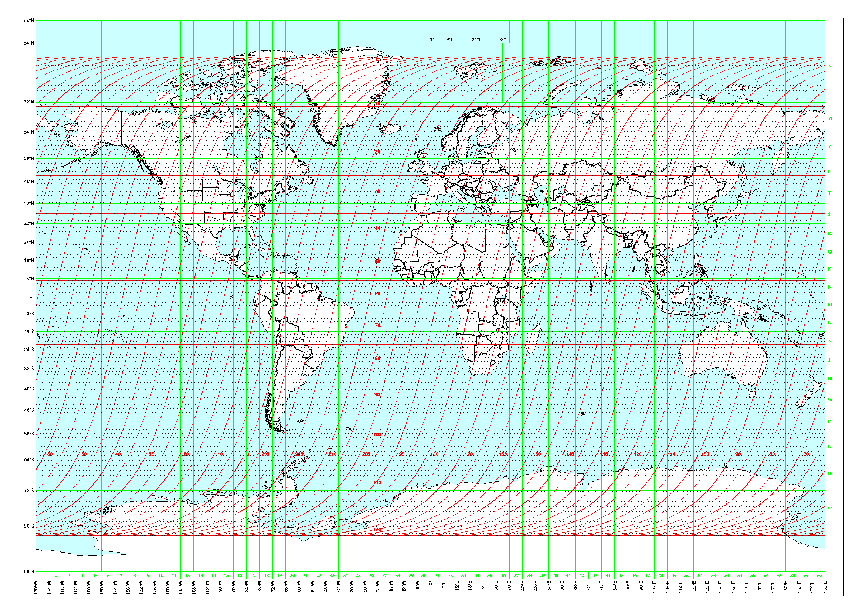
\includegraphics[width=140mm]{eps/landsat_7_wrs2.eps}
  \caption{Map of the Worldwide Reference System-2}
\end{figure}

Landsat 7 Enhanced Thematic Mapper Plus data is available in georeferenced TIFF (GeoTIFF) file format.

Landsat 7 Enhanced Thematic Mapper Plus data is in the public domain in the United States because it is a work of the United States Federal Government under the terms of Title 17, Chapter 1, Section 105 of the Code of Laws of the United States of America.

Landsat 7 ETM+ data can be obtained from: \cite{Terrain-LandsatGLCF, Terrain-LandsatTHN} \\
\url{http://glcf.umd.edu/data/landsat/} \\
\url{http://schorsch.efi.fh-nuernberg.de/data/terrain/Landsat/EarthSat/}

\section{High Resolution Orthoimagery}

\begin{figure}[h!]
  \centering
  
\includegraphics[width=120mm]{eps/usgs_hro_oahu.eps}
  \caption{High Resolution Orthoimagery -- O'ahu Mosaic}
\end{figure}

USGS High Resolution Orthoimagery (HRO) is a collections of aerial photographs with resolution 1 m/pixel or finer, managed and distributed by the USGS EROS Center. Since data came from multiple vendors, resolution, area of coverage, projection, etc. varies.

High Resolution Orthoimagery digital products are distributed in georeferenced TIFF (GeoTIFF) file format.

\begin{figure}[h!]
  \centering
  
\includegraphics[width=120mm]{eps/usgs_hro_honolulu_intl.eps}
  \caption{High Resolution Orthoimagery -- Honolulu International Airport}
\end{figure}

High Resolution Orthoimagery data is in the public domain in the United States because it is a work of the United States Federal Government under the terms of Title 17, Chapter 1, Section 105 of the Code of Laws of the United States of America.

High Resolution Orthoimagery can be obtained from: \cite{Terrain-EarthExplorer} \\
\url{https://earthexplorer.usgs.gov/}

\section{Shuttle Radar Topography Mission}

Shuttle Radar Topography Mission was conducted in February 2000 during STS-99 on board of the Space Shuttle Endeavour. Its purpose was to obtain high resolution digital elevation models of most of the Earth surface.

The Shuttle Radar Topography Mission data is available in two resolutions, 1 arc second resolution (approximately 30 m/pixel) and 3 arc seconds  resolution ( approximately 90 m/pixel).

The Shuttle Radar Topography Mission data is distributed as georeferenced TIFF (GeoTIFF) files arranged into tiles, each covering one degree of latitude and one degree of longitude, named according to their south western corners.

\begin{figure}
  \centering
  
\includegraphics[width=120mm]{eps/srtm_oahu.eps}
  \caption{SRTM Digital Elevation Model -- Greyscale -- O'ahu}
\end{figure}

\begin{figure}
  \centering
  
\includegraphics[width=120mm]{eps/srtm_oahu_shaded.eps}
  \caption{SRTM Digital Elevation Model -- Hillshade -- O'ahu}
\end{figure}

Shuttle Radar Topography Mission data is in the public domain in the United States because it is a work of the United States Federal Government under the terms of Title 17, Chapter 1, Section 105 of the Code of Laws of the United States of America.

Shuttle Radar Topography Mission data can be obtained from:  \cite{Terrain-EarthExplorer} \\
\url{https://earthexplorer.usgs.gov/}

\section{MODIS MOD44W}

\begin{figure}[h!]
  \centering
  
\includegraphics[width=120mm]{eps/mod44w_oahu.eps}
  \caption{MODIS MOD44W Watermask -- O'ahu}
\end{figure}

Moderate Resolution Imaging Spectroradiometer (MODIS) is an imaging sensor on board of the Terra satellite. It was launched by NASA in 1999. MODIS Land Water Mask (MOD44W) is a global raster water mask at 250 m/pixel resolution.

MODIS MOD44W data is available in georeferenced TIFF (GeoTIFF) file format.

MODIS MOD44W data is in the public domain in the United States because it is a work of the United States Federal Government under the terms of Title 17, Chapter 1, Section 105 of the Code of Laws of the United States of America.

MODIS MOD44W watermask data can be obtained from: \cite{Terrain-WaterMaskGLCF} \\
\url{http://glcf.umd.edu/data/watermask/}

\section{Vector Map Level 0}

\begin{figure}[h!]
  \centering
  
\includegraphics[width=120mm]{eps/vmap0_oahu.eps}
  \caption{Vector Map Level 0 -- O'ahu}
\end{figure}

Vector Map Level 0 (VMAP0) provides worldwide coverage of vector-based geospatial data that is equivalent to the 1:1,000,000 scale. [7]

\begin{table}[h!]
  \begin{center}
    \begin{tabular}{ l | l | l }
      \toprule
      \textbf{No.} & \textbf{Name} & \textbf{Coverage} \\ \midrule
      1 & NOAMER   & North America \\
      2 & EURNASIA & Europe and North Asia \\
      3 & SOAMAFR  & South America, Africa and Antarctica \\
      4 & SASAUS   & South Asia and Australia \\
      \bottomrule
    \end{tabular}
    \caption{Vector Map Level 0 Data Sets}
  \end{center}
\end{table}

Vector Map Level 0 data is in the public domain in the United States because it is a work of the United States Federal Government under the terms of Title 17, Chapter 1, Section 105 of the Code of Laws of the United States of America.

NGA Vector Map Level 0 can be obtained from: \cite{Terrain-VMAP0} \\
\url{http://webapp1.dlib.indiana.edu/virtual_disk_library/index.cgi/4911752}

\section{Hawaii Statewide GIS Program}

\begin{figure}[h!]
  \centering
  
\includegraphics[width=120mm]{eps/hawaii_gis_landsat_7.eps}
  \caption{Landsat True-Color Imagery Mosaic}
\end{figure}

State of Hawaii provides geospatial data of Hawaii, including watermask, land cover, satellite true color imagery, elevation data, and more.

Hawaii Statewide GIS Program data can be obtained from: \cite{Terrain-StateOfHawaiiGIS} \\
\url{http://planning.hawaii.gov/gis/download-gis-data/}

\section{Natural Earth and Shaded Relief}

Natural Earth is a public domain map data. Shaded Relief is a repository of public domain cartographic and map data.

Natural Earth data can be obtained from: \cite{Terrain-NaturalEarth}  \\
\url{https://www.naturalearthdata.com/}

Shaded Relief data can be obtained from: \cite{Terrain-ShadedRelief} \\
\url{http://shadedrelief.com/}
